\documentclass[conference]{IEEEtran}
\usepackage{cite}
\usepackage{amsmath,amssymb,amsfonts}
\usepackage{algorithmic}
\usepackage{graphicx}
\usepackage{textcomp}
\usepackage{xcolor}
\usepackage{float}
\usepackage{tikz, pgfplots}
\usepackage{circuitikz}
\def\BibTeX{{\rm B\kern-.05em{\sc i\kern-.025em b}\kern-.08em
    T\kern-.1667em\lower.7ex\hbox{E}\kern-.125emX}}

\pgfplotsset{compat=newest}

\begin{document}

\title{MSP432 Timers, Interrupts, and Analog-to-Digital Converter\\

\author{\IEEEauthorblockN{Tevin Hendess}
\IEEEauthorblockA{\textit{Computer Engineering Department} \\
\textit{Rochester Institute of Technology}\\
Rochester, NY USA \\
twh4619@rit.edu}
\and
\IEEEauthorblockN{Adam Schultzer}
\IEEEauthorblockA{\textit{Computer Engineering Department} \\
\textit{Rochester Institute of Technology}\\
Rochester, NY USA \\
ajs1539@rit.edu}
}
}

\maketitle

\begin{abstract}
The purpose of this exercise was to practice using an opto-isolator to detect changes in the reflection of light within a tube. 
This was accomplished by connecting the OPB745 photo-transducer to the necessary resistors and placing it in the tube and measuring
the voltage and current to see how the values changed as the distance from the sensor to the reflective surface varied. Further tests
were conducted with an inverter introduced into the circuit while the resulting waveform was recorded on an oscilloscope.
\end{abstract}

\section{Design Methodology}

Before constructing the circuit which would be used to test the opto-isolator and measure its output, the correct resistor values
had to be determined from the OPB745 datasheet along with the anticipated voltage values. In doing this, an expected "shape" for the
voltage and current graphs could be determined which allowed for verification as testing was conducted. The resistor value was
calculated according to the equation shown below.

\begin{equation}
    R_F=\frac{5V-V_{LED}}{I_{F_{MAX}}}=\frac{5-1.7}{0.04}=\frac{3.3}{0.04}=82.5\Omega
\end{equation}

As shown in Equation 1, the required resistor value for the LED is 82.5$\Omega$. This value is based on the total voltage through the
circuit (5V) and the voltage drop across the LED (1.7V as specified by the datasheet).

Another important part of the design was determining the expected values and pattern of an output from the photo-transducer. This was
done by examining the OPB745 datasheet which contained a graph of the output current at different distances from the reflective source.
A table of these values is shown in Table \ref{tab:expectedvoltagecurrent}

\begin{table}[H]
    \centering
    \caption{Expected Voltage and Current Values from the OPB745 Datasheet}
    \label{tab:expectedvoltagecurrent}
    \begin{tabular}{|cc|cc|}
    \hline
    \multicolumn{2}{|c|}{}                                                & \multicolumn{2}{c|}{\textbf{$R_{L1}$ = 10k$\Omega$}}                                                                   \\ \hline
    \multicolumn{1}{|c|}{\textbf{Distance (in)}} & \textbf{Distance (mm)} & \multicolumn{1}{c|}{\textbf{$V_{Out}$ (V)}} & \textbf{\begin{tabular}[c]{@{}c@{}}$I_{RL}$\\ (mA)\end{tabular}} \\ \hline
    \multicolumn{1}{|c|}{0.0}                    & 0.0                    & \multicolumn{1}{c|}{2.5}                    & 0.50                                                             \\ \hline
    \multicolumn{1}{|c|}{0.05}                   & 12.7                   & \multicolumn{1}{c|}{6.25}                   & 1.25                                                             \\ \hline
    \multicolumn{1}{|c|}{0.1}                    & 25.4                   & \multicolumn{1}{c|}{6.25}                   & 1.25                                                             \\ \hline
    \multicolumn{1}{|c|}{0.15}                   & 38.1                   & \multicolumn{1}{c|}{5}                      & 1.00                                                             \\ \hline
    \multicolumn{1}{|c|}{0.2}                    & 50.8                   & \multicolumn{1}{c|}{2.5}                    & 0.50                                                             \\ \hline
    \multicolumn{1}{|c|}{0.25}                   & 63.5                   & \multicolumn{1}{c|}{1.25}                   & 0.25                                                             \\ \hline
    \multicolumn{1}{|c|}{0.3}                    & 76.2                   & \multicolumn{1}{c|}{0.85}                   & 0.17                                                             \\ \hline
    \multicolumn{1}{|c|}{0.35}                   & 88.9                   & \multicolumn{1}{c|}{0.75}                   & 0.15                                                             \\ \hline
    \multicolumn{1}{|c|}{0.4}                    & 101.6                  & \multicolumn{1}{c|}{0.65}                   & 0.13                                                             \\ \hline
    \multicolumn{1}{|c|}{0.45}                   & 114.3                  & \multicolumn{1}{c|}{0.55}                   & 0.11                                                             \\ \hline
    \multicolumn{1}{|c|}{0.5}                    & 127                    & \multicolumn{1}{c|}{0.5}                    & 0.10                                                             \\ \hline
    \end{tabular}
\end{table}


With the current values (labeled in Table \ref{tab:expectedvoltagecurrent} as $I_{RL}$), the voltage value can be calculated by simply applying Ohm's Law (V = IR) as the resistance value is also known (10k$\Omega$).

With this information, an expected output graph can be created. This is displayed in Fig.~\ref{fig:expectedvoltage}.
\begin{figure}[htbp]
    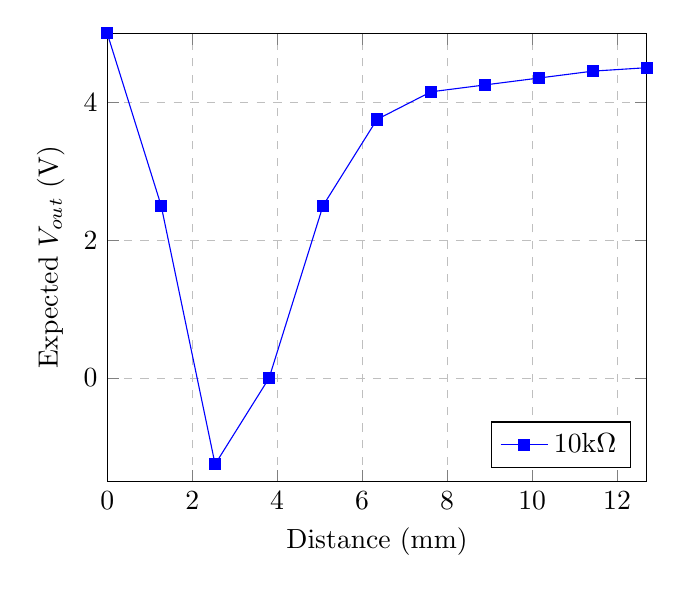
\begin{tikzpicture}
        \begin{axis} [
            xlabel={Distance (mm)},
            ylabel={Expected $V_{out}$ (V)}, % might need to change this
            xmin=0, xmax=12.7,
            ymin=-1.5, ymax=5,
            ymajorgrids=true,
            xmajorgrids=true,
            legend pos=south east,
            grid style=dashed,
        ]
            \addplot[
                color=blue,
                mark=square*
            ]
            coordinates {
                (0, 5)
                (1.27, 2.5)
                (2.54, -1.25)
                (3.81, 0)
                (5.08, 2.5)
                (6.35, 3.75)
                (7.62, 4.15)
                (8.89, 4.25)
                (10.16, 4.35)
                (11.43, 4.45)
                (12.7, 4.5)
            };
            \addlegendentry{10k$\Omega$}
        \end{axis}
    \end{tikzpicture}
    \caption{Distance of Reflective Surface from OPB745 vs Expected Voltage}
    \label{fig:expectedvoltage}
\end{figure}

Fig.~\ref{fig:expectedvoltage} shows what how the output voltage may change as a reflective material is moved further away from the
sensor. The results of an experiment will not exactly match the graph, but should align with the general shape. Of particular
importance is a high starting voltage followed by a steep drop almost immediately which then climbs to maintain a steady value
marginally below the starting supply voltage.

From Table \ref{tab:expectedvoltagecurrent}, the current was also mapped against the distance from the reflective surface.
The resulting plot is shown in Fig.~\ref{fig:expectedcurrent}.

\begin{figure}[htbp]
    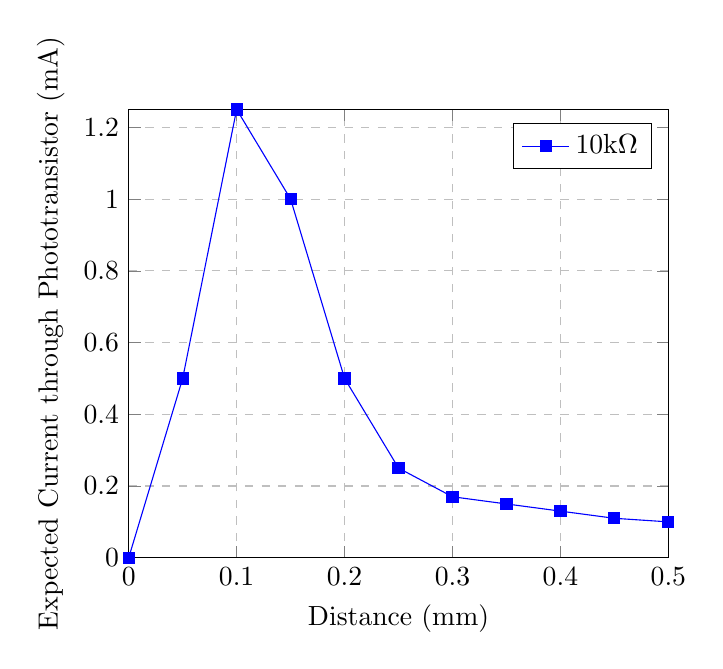
\begin{tikzpicture}
        \begin{axis} [
            xlabel={Distance (mm)},
            ylabel={Expected Current through Phototransistor (mA)}, % might need to change this
            xmin=0, xmax=0.5,
            ymin=0, ymax=1.25,
            ymajorgrids=true,
            xmajorgrids=true,
            legend pos=north east,
            grid style=dashed,
        ]
            \addplot[
                color=blue,
                mark=square*
            ]
            coordinates {
                (0, 0)
                (0.05, 0.5)
                (0.1, 1.25)
                (0.15, 1)
                (0.2, 0.5)
                (0.25, 0.25)
                (0.3, 0.17)
                (0.35, 0.15)
                (0.4, 0.13)
                (0.45, 0.11)
                (0.5, 0.1)
            };
            \addlegendentry{10k$\Omega$}
        \end{axis}
    \end{tikzpicture}
    \caption{Distance of Reflective Surface from OPB745 vs Expected Current}
    \label{fig:expectedcurrent}
\end{figure}

Similarly to Fig.~\ref{fig:expectedvoltage}, it is not expected for the exercise output to exactly match 
Fig.~\ref{fig:expectedcurrent}, however, the general shape is important. The current behaviors inversely to the
voltage and starts at 0 before quickly spiking to a peak before leveling off slightly above 0.

To determine whether the expected results defined in Fig.~\ref{fig:expectedvoltage} and Fig.~\ref{fig:expectedcurrent} would remain true
in a laboratory test, the following circuit was created.

\begin{figure}[!ht]
    \centering
    \resizebox{\linewidth}{!}{%
    \begin{circuitikz}
    \tikzstyle{every node}=[font=\LARGE]
    \draw (6.75,11.75) to[R,l={ \LARGE Rf}] (6.75,9.75);
    \draw (8.5,11.75) to[R,l={ \LARGE 
    RL
    }] (8.5,9.75);
    \draw (3.75,10.5) to[battery ,l={ \LARGE 5V}] (3.75,8.5);
    \draw (6.75,9.25) to[empty photodiode] (6.75,7.25);
    \draw (8.5,7.25) to[Tnpn, transistors/scale=1.19] (8.5,9.25);
    \draw (3.75,7.25) to[short] (4.25,7.25);
    \draw (4.25,7.25) to[short] (8.5,7.25);
    \draw (6.75,9.75) to[short] (6.75,9.25);
    \draw (8.5,9.75) to[short] (8.5,9.25);
    \draw (8.5,11.75) to[short] (3.75,11.75);
    \draw (8.5,9.75) to[short] (11.25,9.75);
    \node [font=\LARGE] at (11,10.25) {Vout};
    \draw (3.75,11.75) to[short] (3.75,10.5);
    \draw (3.75,8.5) to[short] (3.75,7.25);
    \end{circuitikz}
    }%
    \caption{\textit{The Circuit Diagram}}
    \label{fig:circuit_1}
\end{figure}

The circuit in Fig.~\ref{fig:circuit_1} is relatively simple and consists of a 5V power supply placed in parallel with two branches.
The first contains a resistor $R_f$ and the LED side of the photo-transistor. This is what actually emits the light. The resistor is
important as it limits the current flowing through the LED, ensuring that the diode isn't damaged. The value was calculated in
Equation 1. On the second branch, the resistor $R_L$ acts as a load which is connected in series with the transistor side of the
OPB745. It is across this transistor that the voltage defined as "$V_{out}$" is measured.

Slight modifications were made to the circuit in Fig.~\ref{fig:circuit_1} to test the OPB745 with inverters added to the circuit.
This is shown in Fig.~\ref{fig:circuit_2}.

\begin{figure}[!ht]
    \centering
    \resizebox{\linewidth}{!}{%
    \begin{circuitikz}
    \tikzstyle{every node}=[font=\LARGE]
    \draw (6.75,11.75) to[R,l={ \LARGE Rf}] (6.75,9.75);
    \draw (8.5,11.75) to[R,l={ \LARGE 
    RL
    }] (8.5,9.75);
    \draw (3.75,10.5) to[battery ,l={ \LARGE 5V}] (3.75,8.5);
    \draw (6.75,9.25) to[empty photodiode] (6.75,7.25);
    \draw (8.5,7.25) to[Tnpn, transistors/scale=1.19] (8.5,9.25);
    \draw (6.75,9.75) to[short] (6.75,9.25);
    \draw (8.5,9.75) to[short] (8.5,9.25);
    \draw (8.5,11.75) to[short] (3.75,11.75);
    \draw (11,9.75) to[short] (12.25,9.75);
    \node [font=\LARGE] at (12,10.25) {Vout};
    \draw (3.75,11.75) to[short] (3.75,10.5);
    \draw (3.75,8.5) to[short] (3.75,7.25);
    \draw (4.5,6.75) to[square voltage source, sources/symbol/rotate=auto] (4.5,5);
    \draw (4.75,7.25) node[ieeestd not port, anchor=in](port){} (port.out) to[short] (6.5,7.25);
    \draw (port.in) to[short] (4.5,7.25);
    \draw (9.25,9.75) node[ieeestd not port, anchor=in](port){} (port.out) to[short] (11,9.75);
    \draw (port.in) to[short] (9,9.75);
    \draw (9,9.75) to[short] (8.5,9.75);
    \draw (3.75,7.25) to[short] (3.75,5);
    \draw (8.5,7.25) to[short] (8.5,5);
    \draw (4.5,7.25) to[short] (4.5,6.75);
    \draw (6.75,7.25) to[short] (6.25,7.25);
    \draw (3.75,5) to[short] (8.5,5);
    \node [font=\LARGE] at (10,8.75) {74LS14
    };
    \node [font=\LARGE] at (5.5,8) {7406};
    \end{circuitikz}
    }%
    \caption{\textit{The Circuit Diagram with Added Inverters}}
    \label{fig:circuit_2}
\end{figure}

While the circuit in Fig.~\ref{fig:circuit_2} is very similar to that in Fig.~\ref{fig:circuit_1}, two inverters were added along
with a function generator. The location of the voltage probe was not changed relative to the first circuit, but the addition of the
74LS14 chip results in the waveform output being inverted. The second chip, a 7406, is placed in series with the output of the function
generator to invert the input waveform signal.

\section{Results and Analysis}

\subsection{Data Collection}

As a result of testing the circuit with various reflection distances, it was able to be
determined what an ideal testing distance would be, using both a 10k$\Omega$ and 20k$\Omega$ resistance. 
The results of these tests are shown in Table \ref{distanceVoltageCurrent}.

\begin{table}[H]
    \centering
    \caption{Phototransistor Voltage and Current at Various Distances}
    \label{distanceVoltageCurrent}
    \begin{tabular}{|c||c|c||c|c|}
        \hline
         & \multicolumn{2}{c||}{$R_{L1}$ = \textbf{10k}} & \multicolumn{2}{c|}{$R_{L1}$ = \textbf{20k}} \\
        \hline
        Distance & $V_{out}$ (V) & $IRL$ (mA) & $V_{out}$ (V) & $IRL$ (mA) \\
        \hline
        0 &  4.919 &  0.0081 & 4.810 & 0.0095 \\
        1 &  3.175 &  0.1820 & 1.225 & 0.1880 \\
        2 &  0.727 &  0.4261 & 0.737 & 0.2123 \\
        3 &  0.710 &  0.4278 & 0.698 & 0.2142 \\
        4 &  0.729 &  0.4259 & 0.683 & 0.2150 \\
        5 &  0.771 &  0.4217 & 0.687 & 0.2148 \\
        6 &  0.817 &  0.4171 & 0.697 & 0.2143 \\
        7 &  1.652 &  0.3339 & 0.716 & 0.2134 \\
        8 &  2.563 &  0.2430 & 0.735 & 0.2124 \\
        9 &  3.126 &  0.1869 & 0.751 & 0.2116 \\
        10 & 3.420 &  0.1576 & 0.765 & 0.2109 \\
        11 & 3.871 &  0.1126 & 0.790 & 0.2097 \\
        12 & 4.038 &  0.0959 & 0.806 & 0.2089 \\
        13 & 4.217 &  0.0781 & 0.820 & 0.2082 \\
        14 & 4.274 &  0.0724 & 0.880 & 0.2052 \\
        15 & 4.319 &  0.0679 & 1.346 & 0.1820 \\
        20 & 4.576 &  0.0423 & 3.430 & 0.0782 \\
        25 & 4.656 &  0.0343 & 4.078 & 0.0459 \\
        30 & 4.641 &  0.0358 & 4.243 & 0.0377 \\
        35 & 4.580 &  0.0419 & 4.200 & 0.0398 \\
        40 & 4.506 &  0.0493 & 4.043 & 0.0477 \\
        45 & 4.523 &  0.0476 & 4.018 & 0.0489 \\
        50 & 4.585 &  0.0414 & 4.082 & 0.0457 \\
        \hline
    \end{tabular}
\end{table}

Table \ref{distanceVoltageCurrent} demonstrates the relationship between the reflection distance
from the infrared diode to the phototransistor in the optoisolator, and the voltage and current across the
phototransistor. This relationship is slightly different when the circuit contains a 10k$\Omega$ resistor
and a 20k$\Omega$ resistor. The voltage relationships are shown more clearly in Fig.~\ref{distanceVoltageFigure}.

\subsection{Data Visualization and Analysis}

\begin{figure}[htbp]
    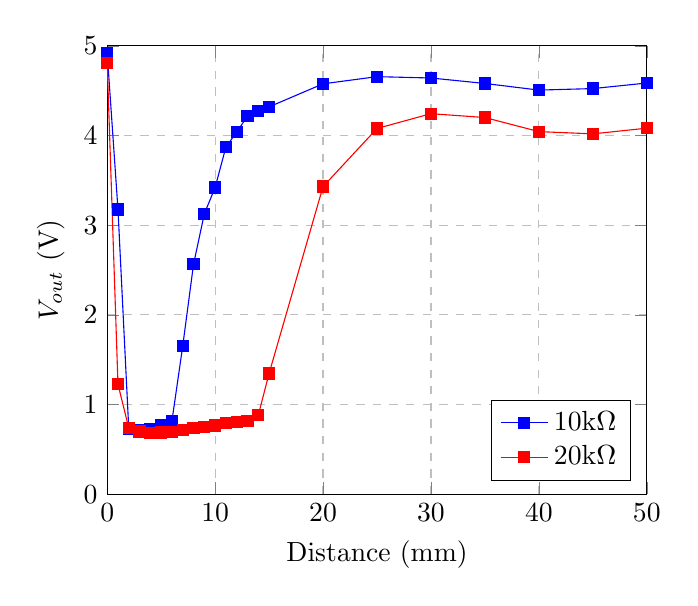
\begin{tikzpicture}
        \begin{axis} [
            xlabel={Distance (mm)},
            ylabel={$V_{out}$ (V)}, % might need to change this
            xmin=0, xmax=50,
            ymin=0, ymax=5,
            ymajorgrids=true,
            xmajorgrids=true,
            legend pos=south east,
            grid style=dashed,
        ]
            \addplot[
                color=blue,
                mark=square*
            ]
            coordinates {
                (0, 4.919)
                (1, 3.175)
                (2, 0.727)
                (3, 0.71)
                (4, 0.729)
                (5, 0.771)
                (6, 0.817)
                (7, 1.652)
                (8, 2.563)
                (9, 3.126)
                (10, 3.42)
                (11, 3.871)
                (12, 4.038)
                (13, 4.216)
                (14, 4.274)
                (15, 4.319)
                (20, 4.576)
                (25, 4.656)
                (30, 4.641)
                (35, 4.58)
                (40, 4.506)
                (45, 4.523)
                (50, 4.585)
            };
            \addlegendentry{10k$\Omega$}

            \addplot[
                color=red,
                mark=square*
            ]
            coordinates {
                (0, 4.81)
                (1, 1.225)
                (2, 0.7372)
                (3,0.6984)
                (4, 0.6831)
                (5, 0.6874)
                (6,0.6971)
                (7, 0.7156)
                (8, 0.735)
                (9, 0.7514)
                (10,0.765)
                (11, 0.7899)
                (12, 0.8059)
                (13, 0.82)
                (14, 0.8802)
                (15, 1.346)
                (20, 3.43)
                (25, 4.078)
                (30, 4.243)
                (35,4.2)
                (40, 4.043)
                (45, 4.018)
                (50, 4.0815)
            };
            \addlegendentry{20k$\Omega$}
        \end{axis}
    \end{tikzpicture}
    \caption{Distance of Reflective Surface from OPB745 vs Voltage}
    \label{distanceVoltageFigure}
\end{figure}

Fig.~\ref{distanceVoltageFigure} shows the voltage in both cases start at near the
logic high voltage and immediately drop, and then rise more
gradually back up to about 0.5 or 1.0 volts lower, for the
10k$\Omega$ case and 20k$\Omega$ case respectively. From these
voltage values, a current relationship could also be calculated
by subtracted $V_{out}$, that being the voltage across the
phototransistor, from the logic high voltage of 5 volts, which
gives the voltage across the resistor, and then using Ohm's law
to determine the current by dividing by the resistance. The
outcome of these calculations is shown in Fig.~\ref{distanceCurrentFigure}

\begin{figure}[htbp]
    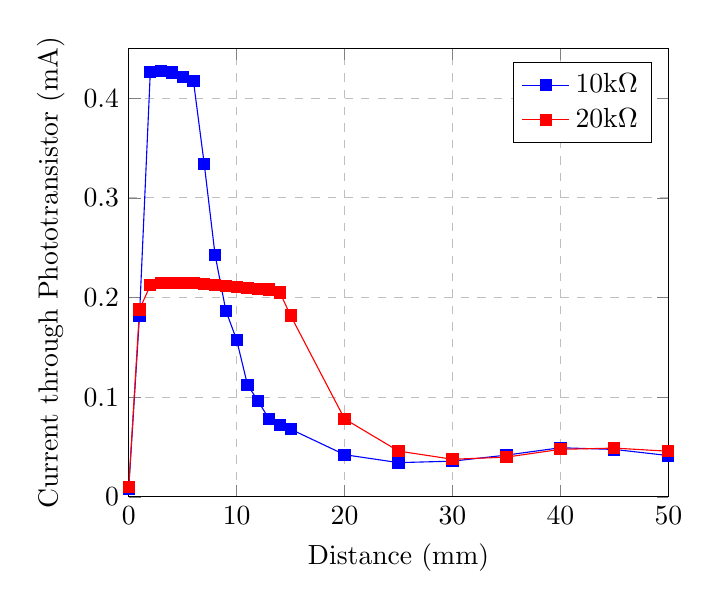
\begin{tikzpicture}
        \begin{axis} [
            xlabel={Distance (mm)},
            ylabel={Current through Phototransistor (mA)},
            xmin=0, xmax=50,
            ymin=0, ymax=0.45,
            ymajorgrids=true,
            xmajorgrids=true,
            legend pos=north east,
            grid style=dashed,
        ]
            \addplot[
                color=blue,
                mark=square*
            ]
            coordinates {
                (0,  0.008077383)
                (1,  0.181990427)
                (2,  0.426106901)
                (3,  0.427802154)                
                (4,  0.425907459)
                (5,  0.421719186)
                (6,  0.41713203 )
                (7,  0.333865178)
                (8,  0.243019545)
                (9,  0.186876745)
                (10, 0.157558835)                
                (11, 0.112584763)
                (12, 0.095931392)
                (13, 0.078111288)
                (14, 0.072397288)
                (15, 0.067909852)
                (20, 0.042281611)
                (25, 0.034303949)
                (30, 0.035799761)
                (35, 0.041882728)                
                (40, 0.049262066)
                (45, 0.047566813)
                (50, 0.041384124)
            };
            \addlegendentry{10k$\Omega$}

            \addplot[
                color=red,
                mark=square*
            ]
            coordinates {
                (0,  0.009462151)      
                (1,  0.187998008)       
                (2,  0.212290837)        
                (3,  0.214223108)        
                (4,  0.21498506 )        
                (5,  0.214770916)        
                (6,  0.214287849)        
                (7,  0.213366534)        
                (8,  0.212400398)       
                (9,  0.211583665)        
                (10, 0.210906375)       
                (11, 0.209666335)        
                (12, 0.208869522)        
                (13, 0.208167331)      
                (14, 0.205169323)        
                (15, 0.181972112)       
                (20, 0.078187251)      
                (25, 0.045916335)       
                (30, 0.037699203)       
                (35, 0.039840637)     
                (40, 0.047659363)       
                (45, 0.048904382)       
                (50, 0.045742032)        
            };
            \addlegendentry{20k$\Omega$}
        \end{axis}
    \end{tikzpicture}
    \caption{Distance of Reflective Surface from OPB745 vs Current}
    \label{distanceCurrentFigure}
\end{figure}

Fig.~\ref{distanceVoltageFigure} and Fig.~\ref{distanceCurrentFigure}
show the relationship between the distance of the reflective
material and the voltage and current associated with the
phototransistor in the OPB745. This data demonstrates three
stages within the relationship. 

When the voltage across the phototransistor is high and
the current through it is low, this means that the phototransistor is
less active, and a low voltage and higher current means
the phototransistor is more active. Therefore, in the first
stage, where the voltage is very high and the current is very
low, it is clear that the phototransistor is receiving almost
no light from the infrared diode. This is due to the fact
that the reflective coating is so close that the light from
the diode cannot escape the OPB745, leading to very little entering
the phototransistor.

In the next stage, the reflective material is far enough
from the OPB745 to allow light to exit, and due to the close
proximity, much is reflected directly into the phototransistor.
This causes the low voltage and high current seen in the data
after the dropoff from the first stage.

When the reflective material is moved far enough from the
device to allow reflected light to scatter to areas
other than the phototransistor, the voltage quickly rises and
the current falls. The values settle at a level that is
less extreme than the initial near-complete occlusion of
the phototransistor, as some light still reaches it.

\subsection{Comparison to Expectations}
The measured outputs of the circuit do not match fully with what was expected based upon
the datasheet of the OPB745. For visual comparison, data from Fig.~\ref{fig:expectedvoltage} and Fig.~\ref{distanceVoltageFigure}
are combined in Fig.~\ref{fig:expectedAndRealVoltage}.

\begin{figure}[htbp]
    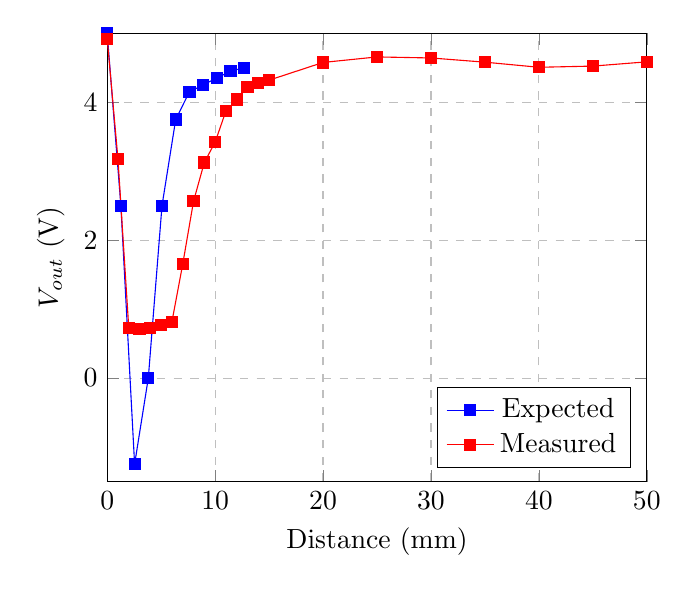
\begin{tikzpicture}
        \begin{axis} [
            xlabel={Distance (mm)},
            ylabel={$V_{out}$ (V)}, % might need to change this
            xmin=0, xmax=50,
            ymin=-1.5, ymax=5,
            ymajorgrids=true,
            xmajorgrids=true,
            legend pos=south east,
            grid style=dashed,
        ]
            \addplot[
                color=blue,
                mark=square*
            ]
            coordinates {
                (0, 5)
                (1.27, 2.5)
                (2.54, -1.25)
                (3.81, 0)
                (5.08, 2.5)
                (6.35, 3.75)
                (7.62, 4.15)
                (8.89, 4.25)
                (10.16, 4.35)
                (11.43, 4.45)
                (12.7, 4.5)
            };
            \addlegendentry{Expected}

            \addplot[
                color=red,
                mark=square*
            ]
            coordinates {
                (0, 4.919)
                (1, 3.175)
                (2, 0.727)
                (3, 0.71)
                (4, 0.729)
                (5, 0.771)
                (6, 0.817)
                (7, 1.652)
                (8, 2.563)
                (9, 3.126)
                (10, 3.42)
                (11, 3.871)
                (12, 4.038)
                (13, 4.216)
                (14, 4.274)
                (15, 4.319)
                (20, 4.576)
                (25, 4.656)
                (30, 4.641)
                (35, 4.58)
                (40, 4.506)
                (45, 4.523)
                (50, 4.585)
            };
            \addlegendentry{Measured}
        \end{axis}
    \end{tikzpicture}
    \caption{Measured and Expected Output Voltages of OPB745}
    \label{fig:expectedAndRealVoltage}
\end{figure}

Fig.~\ref{fig:expectedAndRealVoltage} provides a visual comparison between the measured and expected
outputs of the OPB745 at varying distances from a reflective surface, and demonstrates that there is
a sizable difference between them. There are two primary differences between the graphs, both relating to
the area where most light is reflected. In the expected data, the dip falls to a negative voltage across
the phototransistor, whereas in the measured data, the output voltage only falls to about 0.7 volts. This is
due to the fact that in ideal circumstances, the phototransistor would flow enough current that the voltage
drop across the resistor is greater than 5 volts, leading to a negative current across the phototransistor.
In the real world circuit, loss of light and possible current limiting causes the voltage to stop decreasing before
crossing zero.

The other major difference is the difference in range over which this voltage drop occurs. The OPB745 datasheet
assumes a flat reflective surface, however the aluminum foil used in this setup has a slightly altered affect.
This may be due to a slightly convex circuit allowing a greater range of distances to reflect light in the
correct spot. Although it appears that the bottom of the voltage drop has a flat response over this section
from approximately 2mm to 6mm, it may be that the voltage would have gone lower and was only stopped by
the phototransistor's physical characteristics, and so does not necessarily imply a steady amount of light
received by the phototransistor.

\subsection{Usage with Digital Logic}

In order for the OPB745 to be used as an isolator in a digital
circuit, the output must be interpreted as a digital signal.
This was done by passing the output through an 74LS14 
Schmitt-trigger inverter, as
well as feeding the input diode with the output of an 7406
inverter. In steady state with working components, this circuit
will behave as intended. However, due to the partially analog
nature of the circuit, there is a switching frequency where
this correct digital behavior begins to break down. The circuit
was fed with a switching signal with both the input and output voltage
monitored by a oscilloscope. The maximum operable frequencies using
10k$\Omega$ and 20k$\Omega$ resistors were
recorded in their working state and shown in Fig.~\ref{fig:maxFreq10k} and Fig.~\ref{fig:maxFreq20k} respectively.

\begin{figure}[!ht]
    \centering
    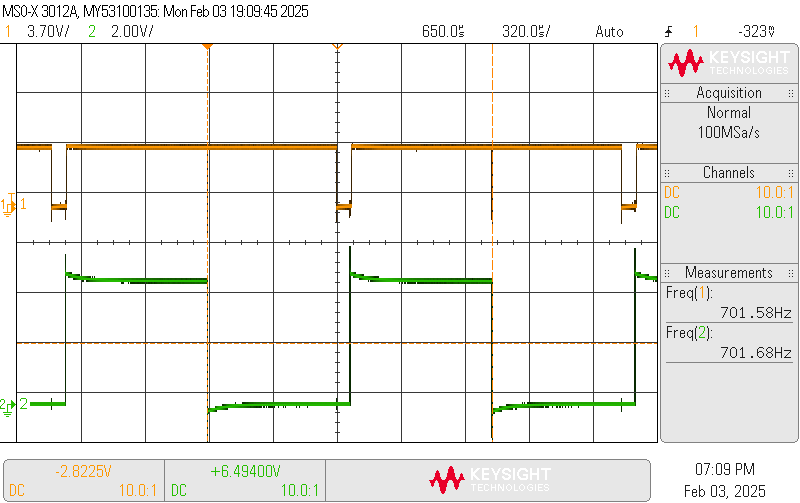
\includegraphics[width=\linewidth]{images/10k Before Good.png}
    \caption{\textit{Maximum Switchable Frequency with 10k$\Omega$ Resistor}}
    \label{fig:maxFreq10k}
\end{figure}

\begin{figure}[!ht]
    \centering
    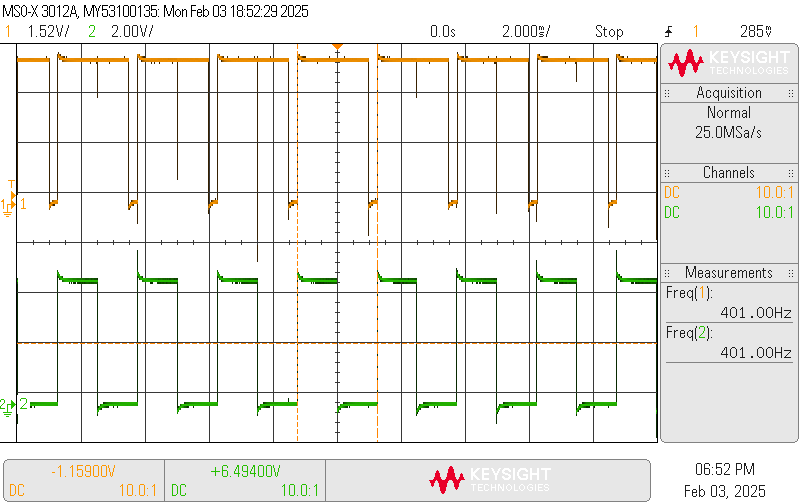
\includegraphics[width=\linewidth]{images/20k Before.png}
    \caption{\textit{Maximum Switchable Frequency with 20k$\Omega$ Resistor}}
    \label{fig:maxFreq20k}
\end{figure}

Fig.~\ref{fig:maxFreq10k} demonstrates that the circuit with the 10k$\Omega$
resistor operated at a maximum frequency of about 700Hz, while Fig.~\ref{fig:maxFreq20k}
demonstrates that the circuit with the 20k$\Omega$ resistor could operate at only 400Hz.

\section{Questions}

\subsection{In the lab we do not use a 7406 inverter on the output; instead we use the 74LS14 with Schmitt
trigger. Why do we need to do this, and what is the difference between the two?}

We need to use the 74LS14 to provide additional protection against noise on the output, as it
prevents multiple edges from being produced from a signal crossing a threshold voltage. It does this
by switching to high and low outputs at diffenent input voltages, leaving something like a voltage dead-zone,
where changes in voltage up or down will only affect the output after reaching a certain point past the middle
of the voltage range. This dead-zone is refered to as the hysteresis region. The 7406 is not a Schmitt trigger
and does not have a hysteresis region, only a single threshold voltage, making the output voltages entirely
defined by the current input.

\subsection{Why does the voltage start at ~5V at 0mm and then drop quickly? Why does it eventually go
back to ~5V?}

The voltage starts at about 5V due to the fact that the
phototransistor is nearly completely off at 0mm. This is
because when the reflective material is fully pressed against
the OPB745, it blocks both the infrared diode from emitting
light outside the device, and blocks the phototransistor from
receiving any light. Once the material is moved back a small amount, the
infrared light can be reflected most effectively to the
phototransistor, turning it on and decreasing the voltage
across it. When the material continues to be moved further 
back, a point is crossed where the light begins to be scattered
to other locations and becomes less focused on the
phototransistor, leading the phototransistor to turn on less,
flowing less current, and therefore for the voltage over the
component to gradually increase.

\subsection{Why does the frequency change when going from a 10k$\Omega$ load resistor to a 20k$\Omega$ load resistor?
Did you anticipate it increasing or decreasing and why?}

When doubling the size of the load resistor from 10k$\Omega$  to 20k$\Omega$, the frequency changes because the transistor is recieving
less voltage as more is being lost across the resistor. As a result of the lower voltage, the transistor has less range to decipher
whether the incoming signal is high or low on the square wave. With more voltage, faster frequencies are less damaging to the results as
the actual signal can still be detected. It is expected, therefore, that the circuit with the 20k$\Omega$ load resistor will break down
at a slower frequency than the circuit with the 10k$\Omega$ is able to achieve.

\section{Conclusion}
Through the course of this exercise, the properties of the OPB745 were shown and its behavior was compared between a laboratory
setting and the expected values shown on the datasheet. Because the measured results of the tests showed similar characteristics and
patterns to that of the datasheet's values, the exercise can be deemed a success. In the future, the OPB745 can be used to detect changes
in an environment without requiring contact, something which will be immensely helpful in developing autonomous car technology. It was
necessary, however, to understand how the device functions before it could be put to use in more specialized applications.

\end{document}
